\section{Pokrývání}
\subsection{Nezávislé množiny, nezávislost}\label{nezavislost}
Mějme graf $G = (V,E) \in \S$. Množinu vrcholů $A \subseteq V$ nazveme \ii{nezávislou množinou}, jestliže v grafu
neexistuje hrana s oběma krajními vrcholy v $A$. 

\ii{Nezávislost grafu}, značíme ji $\alpha_0(G)$, je rovna počtu vrcholů v nejpočetnější nezávislé množině v $G$.
\begin{figure}[H]
    \centering
    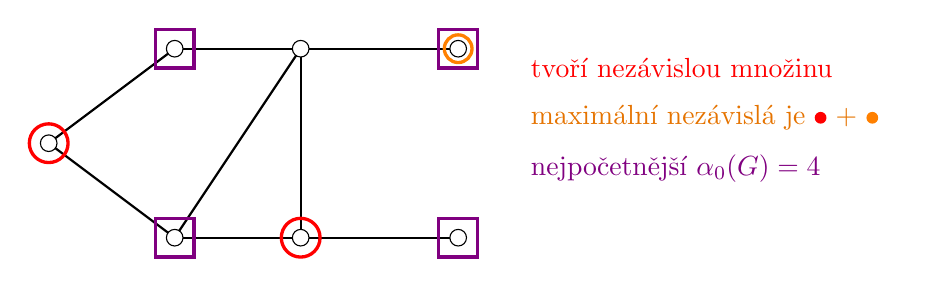
\begin{tikzpicture}[
        scale=0.8,
        auto,
        vertex/.style={circle, draw=black, fill=white, minimum size=6pt, inner sep=0pt},
        edge/.style={thick, black, line cap=round},
        hl_red/.style={circle, draw=red, very thick, minimum size=14pt, outer sep=2pt},
        hl_purple/.style={rectangle, draw=violet, very thick, minimum size=14pt, outer sep=2pt},
        hl_orange/.style={circle, draw=orange, very thick, minimum size=10pt},
    ]

        \coordinate (v1) at (0, 1.5);
        \coordinate (v2) at (2, 3);
        \coordinate (v3) at (2, 0);
        \coordinate (v4) at (4, 3);
        \coordinate (v5) at (4, 0);
        \coordinate (v6) at (6.5, 3);
        \coordinate (v7) at (6.5, 0);

        \draw[edge] (v1) -- (v2);
        \draw[edge] (v1) -- (v3);
        \draw[edge] (v2) -- (v4);
        \draw[edge] (v3) -- (v5);
        \draw[edge] (v3) -- (v4);
        \draw[edge] (v4) -- (v5);
        \draw[edge] (v4) -- (v6);
        \draw[edge] (v5) -- (v7);

        \node[hl_red] at (v1) {};
        \node[hl_red] at (v5) {};

        \node[hl_purple] at (v2) {};
        \node[hl_purple] at (v3) {};
        \node[hl_purple] at (v6) {};
        \node[hl_purple] at (v7) {};

        \node[hl_orange] at (v6) {};

        \foreach \point in {v1,v2,v3,v4,v5,v6,v7} {
            \node[vertex] at (\point) {};
        }

        \begin{scope}[xshift=7.5cm, yshift=1.5cm, every node/.style={right, align=left}]
            \node[text=red] at (0, 1.2) {tvoří nezávislou množinu};

            \node[text=orange!90!black] at (0, 0.4) {
                maximální nezávislá je \tikz[baseline=-0.6ex]\node[circle, fill=red, inner sep=1.5pt]{};
                + \tikz[baseline=-0.6ex]\node[circle, fill=orange, inner sep=1.5pt]{};
            };

            \node[text=violet] at (0, -0.4) {nejpočetnější $\alpha_0(G)=4$};
        \end{scope}
    \end{tikzpicture}
\end{figure}

\subsection{Vrcholové pokrytí}\label{vrchPok}
Je dán prostý neorientovaný $G = (V,E) \in \S$. Množina vrcholů $K \subseteq V$ se nazývá \ii{vrcholové pokrytí}, 
jestliže každá hrana $e \in E$ má alespoň jeden krajní vrchol v $K$.

Počet vrcholů v nejméně početném vrcholovém pokrytí v grafu $G$ značíme $\beta_0(G)$.

Jestliže $K$ je vrcholové pokrytí a $K \subseteq K^\prime$, tak $K^\prime$ je také vrcholové pokrytí.
\begin{figure}[H]
    \centering
    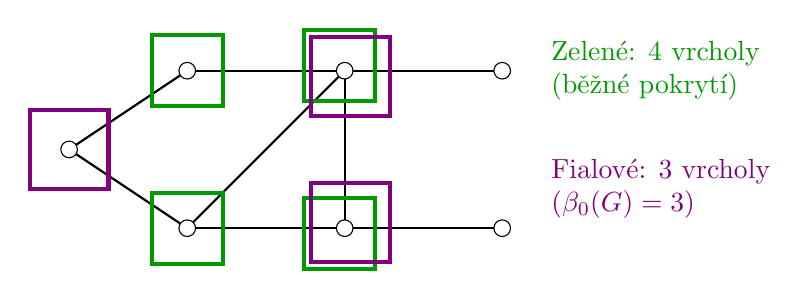
\begin{tikzpicture}[
        vertex/.style={circle, draw=black, fill=white, minimum size=6pt, inner sep=0pt},
        edge/.style={thick, black, line cap=round},
        green_cover/.style={draw=green!60!black, line width=1.5pt, minimum size=9mm, rectangle},
        purple_cover/.style={draw=violet, line width=1.5pt, minimum size=10mm, rectangle}
    ]

        \node[vertex] (v1) at (0, 1) {};
        \node[vertex] (v2) at (1.5, 2) {};
        \node[vertex] (v7) at (1.5, 0) {};
        \node[vertex] (v3) at (3.5, 2) {};
        \node[vertex] (v6) at (3.5, 0) {};
        \node[vertex] (v4) at (5.5, 2) {}; 
        \node[vertex] (v5) at (5.5, 0) {};

        \draw[edge] (v1) -- (v2);
        \draw[edge] (v1) -- (v7);
        \draw[edge] (v2) -- (v3);
        \draw[edge] (v7) -- (v6);
        \draw[edge] (v3) -- (v7);
        \draw[edge] (v3) -- (v6);
        \draw[edge] (v3) -- (v4);
        \draw[edge] (v6) -- (v5);

        \node[green_cover] at (v2) {}; 
        \node[green_cover] at (v7) {};
        \node[green_cover, shift={(-2pt, 2pt)}] at (v3) {};
        \node[green_cover, shift={(-2pt, -2pt)}] at (v6) {};

        \node[purple_cover] at (v1) {};
        \node[purple_cover, shift={(2pt, -2pt)}] at (v3) {};
        \node[purple_cover, shift={(2pt, 2pt)}] at (v6) {};

        \node[right, align=left, text=green!60!black] at (6, 2) {Zelené: 4 vrcholy\\(běžné pokrytí)};
        \node[right, align=left, text=violet] at (6, 0.5) {Fialové: 3 vrcholy\\($\beta_0(G) = 3$)};
    \end{tikzpicture}    
\end{figure}

\subsection{Věta o vztahu vrcholového pokrytí a nezávislosti}
Je dán prostý neorientovaný graf $G = (V,E)$ bez smyček s $n$ vrcholy. Platí
\begin{equation}
    \alpha_0(G) + \beta_0(G) = n.
\end{equation}
\dukaz Máme $G = (V,E) \in \S$. $|V| = n$.\\
\enquote{$\geq$}: Uvažujme $N$ nezávislou, $|N| = \alpha_0(G)$. Pak $V \setminus N$ je \hyperref[vrchPok]{vrcholové 
pokrytí}. Což znamená
\begin{equation}
    |V \setminus N| = n - \alpha_0(G) \geq \beta_0(G).
\end{equation}
Takže
\begin{equation}
    n \geq \alpha_0(G) + \beta_0(G).
\end{equation}
\enquote{$\leq$}: Uvažujme vrcholové pokrytí $K$ s $|K| = \beta_0(K)$. Pak $V \setminus K$ je 
\hyperref[nezavislost]{nezávislá} množina. A
\begin{equation}
    |V \setminus K| = n - \beta_0(G) \leq \alpha_0(G).
\end{equation}
Tudíž
\begin{equation}
    n \leq \alpha_0(G) + \beta_0(G).
\end{equation}

Dostáváme tedy 
\begin{equation}
    n = \alpha_0(G) + \beta_0(G).
\end{equation}
\hspace{\fill}\qed

\subsection{Hranové pokrytí}\label{hranPok}
Je dán prostý neorientovaný graf $G = (V,E)$ bez smyček a izolovaných vrcholů. Množina hran $B \subseteq E$ se nazývá 
\ii{hranové pokrytí}, jestliže každý vrchol je krajním vrcholem alespoň jedné hrany z $B$.

Definujme $\beta_1(G)$ jako počet hran v nejméně početném hranovém pokrytí.
\begin{figure}[H]
    \centering
    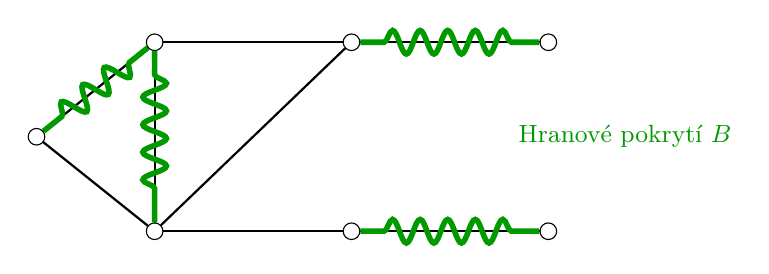
\begin{tikzpicture}[
        vertex/.style={circle, draw=black, fill=white, minimum size=6pt, inner sep=0pt},
        edge/.style={thick, black, line cap=round},
        edge_cover/.style={
            draw=green!60!black, 
            line width=2pt, 
            decorate, 
            decoration={snake, amplitude=1.5mm, segment length=3.5mm, pre length=3mm, post length=3mm}
        }
    ]

        \node[vertex] (v1) at (0, 1) {};
        \node[vertex] (v2) at (1.5, 2.2) {};
        \node[vertex] (v7) at (1.5, -0.2) {};
        \node[vertex] (v3) at (4, 2.2) {};
        \node[vertex] (v6) at (4, -0.2) {};
        \node[vertex] (v4) at (6.5, 2.2) {};
        \node[vertex] (v5) at (6.5, -0.2) {};

        \draw[edge] (v1) -- (v2);
        \draw[edge] (v1) -- (v7);
        \draw[edge] (v2) -- (v7);
        
        \draw[edge] (v2) -- (v3);
        \draw[edge] (v3) -- (v7);
        \draw[edge] (v7) -- (v6);
        
        \draw[edge] (v3) -- (v4);
        \draw[edge] (v6) -- (v5);
        
        \draw[edge_cover] (v1) -- (v2);
        \draw[edge_cover] (v2) -- (v7);
        \draw[edge_cover] (v3) -- (v4);
        \draw[edge_cover] (v6) -- (v5);

        \node[right, align=left, text=green!60!black, font=\small] at (6, 1) 
            {Hranové pokrytí $B$};
    \end{tikzpicture}
\end{figure}

\subsection{Věta o vztahu hranového pokrytí a maximálního párování}
Je dán prostý neorientovaný graf $G = (V,E) \in \S$ bez izolovaných vrcholů s $n$ vrcholy. Pak platí
\begin{equation}
    \alpha_1(G) + \beta_1(G) = n,
\end{equation}\vspace{-0.5em}
kde $\alpha_1$ je počet hran v maximálním párování grafu $G$ (tj. $\alpha_1(G) = P_{\max}$).\\
\dukaz\\
\enquote{$\leq$}: Vezmeme nejméně početné \hyperref[hranPok]{hranové pokrytí} $B \subseteq E$.
Jak vypadají komponenty souvislosti $(U,B)$?
\begin{figure}[H]
    \centering
    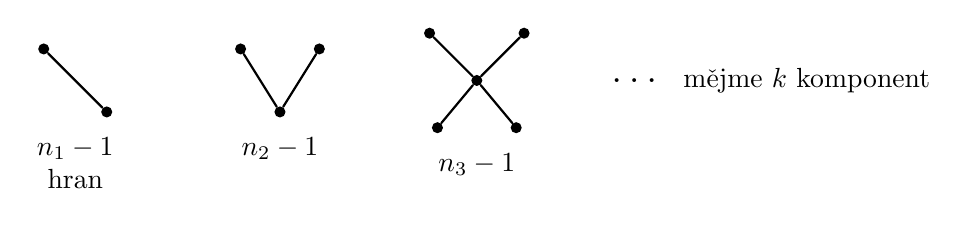
\begin{tikzpicture}[
        scale=1,
        vertex/.style={circle, fill=black, minimum size=4pt, inner sep=0pt},
        edge/.style={thick, draw=black, line cap=round}
    ]

        \node[vertex] (c1_1) at (0, 1) {};
        \node[vertex] (c1_2) at (0.8, 0.2) {};
        \draw[edge] (c1_1) -- (c1_2);
        
        \node[below, align=center, yshift=-0.2cm] at (0.4, 0.2) {$n_1 - 1$\\hran};

        \begin{scope}[shift={(2.5,0)}]
            \node[vertex] (c2_center) at (0.5, 0.2) {};
            \node[vertex] (c2_1) at (0, 1) {};
            \node[vertex] (c2_2) at (1, 1) {};
            
            \draw[edge] (c2_1) -- (c2_center) -- (c2_2);
            
            \node[below, yshift=-0.2cm] at (0.5, 0.2) {$n_2 - 1$};
        \end{scope}

        \begin{scope}[shift={(5.5,0)}]
            \node[vertex] (c3_center) at (0, 0.6) {};
            \node[vertex] (c3_1) at (-0.6, 1.2) {};
            \node[vertex] (c3_2) at (0.6, 1.2) {};
            \node[vertex] (c3_3) at (-0.5, 0) {};
            \node[vertex] (c3_4) at (0.5, 0) {};
            
            \draw[edge] (c3_center) -- (c3_1);
            \draw[edge] (c3_center) -- (c3_2);
            \draw[edge] (c3_center) -- (c3_3);
            \draw[edge] (c3_center) -- (c3_4);
            
            \node[below, yshift=-0.2cm] at (0, 0) {$n_3 - 1$};
        \end{scope}

        \node at (7.5, 0.6) {\Large $\dots$};
        \node[right, align=left] at (8, 0.6) {mějme $k$ komponent};
    \end{tikzpicture}
\end{figure}
Takže 
\begin{equation}
    \beta_1 = |B| = \underbrace{n_1 + n_2 + \dots + n_k}_{n} - k = n-k.    
\end{equation}
Mějme párování $P$, kde z každé komponenty souvislosti vezmeme jednu libovolnou hranu, takže $|P| = k$. Tedy máme 
$b_1(G) = n-k$ a $|P| = k \leq \alpha_1(G)$.
\begin{align}
    n = \beta_1(G) + k &\leq \beta_1(G) + \alpha_1(G) \\
    n &\leq \alpha_1(G) + \beta_1(G)
\end{align}
\enquote{$\geq$}: Mějme $P_{\max}$, párování s $|P_{\max}| = \alpha_1(G)$.
\begin{figure}[H]
    \centering
    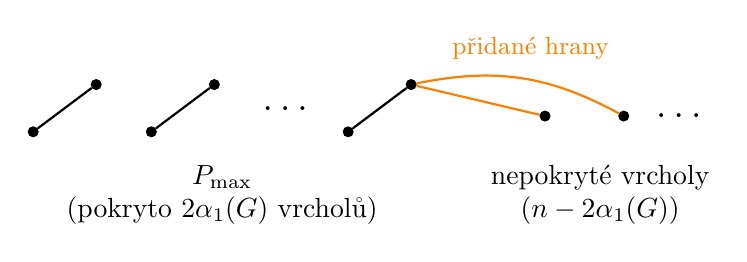
\begin{tikzpicture}[
        scale=1,
        vertex/.style={circle, fill=black, minimum size=4pt, inner sep=0pt},
        edge/.style={thick, draw=black, line cap=round},
        added/.style={thick, draw=orange, line cap=round}
    ]

        \node[vertex] (p1_a) at (0, 0) {};
        \node[vertex] (p1_b) at (0.8, 0.6) {};
        \draw[edge] (p1_a) -- (p1_b);

        \node[vertex] (p2_a) at (1.5, 0) {};
        \node[vertex] (p2_b) at (2.3, 0.6) {};
        \draw[edge] (p2_a) -- (p2_b);

        \node at (3.2, 0.3) {\Large $\dots$};

        \node[vertex] (p3_a) at (4.0, 0) {};
        \node[vertex] (p3_b) at (4.8, 0.6) {};
        \draw[edge] (p3_a) -- (p3_b);

        \node[vertex] (u1) at (6.5, 0.2) {};
        \node[vertex] (u2) at (7.5, 0.2) {};
        \node at (8.2, 0.2) {\Large $\dots$};

        \draw[added] (p3_b) -- (u1);
        \draw[added] (p3_b) to[bend left=20] (u2);

        \node[below, align=center, yshift=-0.3cm] at (2.4, 0) {$P_{\max}$\\(pokryto $2\alpha_1(G)$ vrcholů)};
        \node[below, align=center, yshift=-0.3cm] at (7.2, 0) {nepokryté vrcholy\\($n - 2\alpha_1(G)$)};
        
        \node[text=orange, font=\small, anchor=south west] at (5.2, 0.8) {přidané hrany};
    \end{tikzpicture}
\end{figure}
$B = P_{\max} \cup \textcolor{orange}{\bc{e \mid e \text{ je přidaná}}}$.
\begin{align}
    |B| = \alpha_1(G) + n - 2\alpha_1(G) = n-\alpha_1(G) &\geq \beta_1(G) \\
    n &\geq \alpha_1(G) + \beta_1(G)
\end{align}

Dostáváme tedy
\begin{equation}
    n = \alpha_1(G) + \beta_1(G).
\end{equation}
\hspace{\fill}\qed
